
\section{Tutorial}
\label{section:tutorial}
\setcounter{footnote}{0}

Here's a tutorial walk-through of some how to use \rscape. This should
suffice to get you started.

\subsection {Modes of \rscape}

\begin{tabular}{ll}
\multicolumn{2}{c}{\textbf{MSA input with annotated consensus secondary structure}} \\ 
 & \\ 
\textbf{R-scape}   & Reports all pairs which covariation scores have E-values smaller or equal to a target E-value.\\
\textbf{}          & Draws the given consensus structure annotated with the significantly covarying base pairs.\\
 & \\ 
\multicolumn{2}{c}{\textbf{MSA input without an annotated secondary structure}}  \\
 & \\ 
\textbf{R-scape}   & Reports all pairs which covariation scores have E-values smaller or equal to a target E-value.\\
\textbf{}          & Builds the best consensus structure that includes all significantly covarying pairs,\\
\textbf{}          & \hspace{5mm}\emph{the maximum-covariation optimal consensus structure}.\\
\textbf{}          & Draws the \emph{maximum-covariation optimal consensus structure} annotated with the significantly \\
\textbf{}          & \hspace{5mm}covarying base pairs.\\
 & \\ 
\end{tabular} \\
\\

In the Tutorial section, I'll show examples of running each \rscape,
using examples in the \ccode{tutorial/} subdirectory of the
distribution.


\subsection{Files used in the tutorial}

The subdirectory \prog{/tutorial} in the \rscape\ distribution contains the
files used in the tutorial. 

The tutorial provides several examples of RNA structural
alignments, all in Stockholm format:

\begin{sreitems}{\emprog{updated\_Arisong.sto}}
\item[\emprog{updated\_Arisong.sto}] Structural alignment of the ciliate
  Arisong RNA. This alignment is an updated
  version of the one published in~\citep{JungEddy11}.
\item[\emprog{ar14.sto}] Structural alignment of the $\alpha$-proteobacteria ncRNA ar14. This alignment is an updated version of the one
  published in~\citep{delVal12}.
\item[\emprog{RF00005.sto}] Rfam v12.0~\citep{Nawrocki15} seed alignment of tRNA. 
\item[\emprog{RF00001-noss.sto}] Rfam v12.0 seed alignment of 5S rRNA, after removing the consensus secondary structure. 
\end{sreitems}


\subsection{Running \rscape\, on one alignment file}
To run \rscape\ with default parameters on alignment file
\prog{tutorial/updated\_Arisong.sto} use:\\

\user{bin/R-scape tutorial/updated\_Arisong.sto}\\

\noindent
The output is a list of the signifcantly covarying positions

\begin{sreoutput}
# R-scape :: RNA Structural Covariation Above Phylogenetic Expectation
# R-scape 0.1 (FEB 2016)
# Copyright (C) 2016 Howard Hughes Medical Institute.
# Freely distributed under the GNU General Public License (GPLv3).
# - - - - - - - - - - - - - - - - - - - - - - - - - - - - - - - - - - - -
# MSA updated_Arisong_1 nseq 69 (95) alen 65 (150) avgid 65.16 (64.97) nbpairs 20 (20)
# Method Target_E-val cov_at_target_E-val [cov_min,conv_max] [FP | TP True Found | Sen PPV F] 
# GTp    0.05         41.31               [-9.74,89.08]      [2 | 9 20 11 | 45.00 81.82 58.06] 
#       left_pos       right_pos        score   E-value
#------------------------------------------------------------
*	      98	     106	89.08	0
*	     122	     137	69.00	0
*	      96	     108	65.95	0
*	     120	     139	56.32	0
 	     104	     130	47.18	5.99449e-12
*	     119	     140	43.84	6.01567e-06
 	      93	     104	43.65	6.01567e-06
*	      94	     110	43.17	4.29923e-05
*	     124	     134	42.97	0.000111963
*	     123	     135	41.95	0.00405659
*	     121	     138	41.92	0.00405659
\end{sreoutput}
The ``*'' in the first column indicates that the pair is part of the
annotated structure in the \prog{updated\_Arisong.sto} file. A blank
indicates a pair that is not compatible with the structure. A ``~``
indicated an interaction not in the annotated structure but compatible
with it (none in this example).

\subsection{Default parameters}

Default parameters are:

\begin{sreitems}{\emprog{Pairwise percent identity:}}
\item[\emprog{Target E-value:}]default is 0.05. \rscape\, reports
  pairs which covariation score has E-value smaller or equal to the
  target value.  The target E-value can be changed with option
  \emprog{-E <x>}, $x >= 0$.

\item[\emprog{Pairwise percent identity:}]Sequences with more than
  97\% similarity to each other are removed.  Pairwise \% identity is
  defined as the ratio of identical positions divided by the minimum
  length of the two sequences. The maximum pairwise percentage
  identity in the alignment can be changed with option \emprog{-I
    <x>}, $0<x<=1$.

\item[\emprog{Gaps in columns}]Columns with more than 50\% gaps are
  removed. The gap threshold for removing columns can be modified
   using option \emprog{--gapthresh <x>} , $0<x<=1$.

 \item[\emprog{Covariation statistic}]The default covariation statistic
   is the product-average corrected G-Test (equivalent to option
   \emprog{--GTp}).

 \item[\emprog{Covariation Class}]\rscape\ uses the 16 component
   covariation statistic (C16), unless the number of sequences in the
   alignment is $\leq$ 8 or the length of the alignment is $\leq$ 50,
   in which case it uses the two-class covariation statistic (C2). A
   particular covariation class can be selected using either
   \emprog{--C16} or \emprog{--C2}.

   The threshold for the minimum number of sequences can be changed
   with option \prog{--nseqthresh <n>}.  The threshold for the minimun
   alignment length can be changed with option \prog{--alenthresh <n>}.

 \item[\emprog{Null alignments:}]\rscape\ in order to estimate E-values
   produces 20 null alignments, unless the product of the number of
   sequences by the length of the alignment $<$ 10,000 in which case
   the number of null alignments is 50; or $<$ 1,000 in which case it
   is 100. The number of null alignments can be controlled with option
   \emprog{--nshuffle <n>}.
 \end{sreitems}

 A full list of the \rscape\ options is fund by using

 \user{\rscape\ -h}

 \subsection{Tabular output per input file}

 The output file \emprog{tutorial/updated\_Arisong.out} looks like this:

 \begin{sreoutput}
 # MSA updated_Arisong_1 nseq 69 (95) alen 65 (150) avgid 65.16 (64.97) nbpairs 20 (20)
 # Method Target_E-val cov_at_target_E-val [cov_min,conv_max] [FP | TP True Found | Sen PPV F] 
 # GTp    0.05         41.31               [-9.74,89.08]     [2 | 9 20 11 | 45.00 81.82 58.06] 
                 93             104      43.65   6.01567e-06
 *               94             110      43.17   4.29923e-05
 *               96             108      65.95   0
 *               98             106      89.08   0
 ...
 \end{sreoutput}
 The output file is a tabular list of significant pairs ordered by the first positions:

 \begin{sreitems}{\prog{Second and third columns}}
 \item[\prog{First column}] indicates whether the significant pair is
   part of the given structure (*), or not.  If the pair is not in the
   structure, we distinguish whether the pair is compatible with the
   given structure ($\sim$) o not, in which case it is a blank.

 \item[\prog{Second and third columns}] are the two positions of the
   pair, $i\leq j$ respectively. Positions are relative to the input
   alignment.

 \item[\prog{Forth column}] is the covariation score

 \item[\prog{Fifth column}] is the E-value. Significant positions
   have E-values $<< 1$.
 \end{sreitems}
 The output file also includes two comment lines per alignment in the
 file:

 \begin{sreitems}{\prog{Second comment line}}
 \item[\prog{First comment line}]describes properties of the
   alignment: number of sequence (nseq), alignment length (alen),
   average percentage identity (avgid), and number of base pairs
   (nbpairs).  Values in parenthesis correspond to the alignment as is
   given. Values not in parenthesis correspond to the analyzed
   alignment after the default filters have been applied.

 \item[\prog{Second comment line}]describes properties of the
   \rscape\ search: the covariation method (GTp), the E-value threshold
   (0.05), the score at that E-value (42.3), the range of scores for all
   pairs in the alignments (from -9.7 to 89.1), the number of covarying
   not base pairs (2), the number of covarying base pairs (9), the
   number of base pairs (20), and the total number of covarying pairs
   (11). Lastly we provide the sensitivity (SEN=45.0=9/20), positive
   predictive value (PPV=81.8=9/11), and F-measure (F=58.1 = 2 * SEN *
   PPV / (SEN+PPV)).
 \end{sreitems}


 \subsection{Outputs per alignment}
 Two files are produced per alignment in the input file: \\

 File \emprog{tutorial/updated\_Arisong\_1.R2R.sto} is a Stockholm
 formatted alignment that includes the input alignment annotated with
 the consensus structure. This Stockholm file also includes the
 additional annotation required to use the drawing program R2R.

 It is possible that the resulting drawing will show parts of the
 secondary structure occluded from each other (especially for long
 RNAs).  Using this file, one can customize a different drawing of the
 structure using the R2R documentation, provided in
 \prog{lib/R2R/R2R-manual.pdf}.\\

 File \emprog{tutorial/updated\_Arisong\_1.his} looks like this:
 \begin{sreoutput}
 more tutorial/updated_Arisong.his
 89.046301       0.000480769
 68.879658       0.000961538
 65.816370       0.00144231
 56.115959       0.00192308
 ...
 &
 41.054795       9.61538e-06
 40.799521       3.84615e-05
 40.288973       6.73077e-05
 ...
 &
 49.478836       2.13504e-20
 49.223562       4.27009e-20
 48.968288       1.06752e-19
 ...
 &
 \end{sreoutput}
 The first column is a covariation score (x). The second column is the
 survival function $P(X > x)$, that is the frequency of pairs having
 score larger than x. The file includes three histograms separated by a
 ``\&'' line. The three histogram correspond to:

 \begin{sreitems}{\prog{Second histogram}}
 \item[\prog{First histogram}] the given alignment, all possible pairs.
 \item[\prog{Second histogram}] the aggregation of all null alignments, all possible pairs.
 \item[\prog{Third histogram}] the expected null histogram according to the tail Gamma fit.
 \end{sreitems}


 \subsection{Graphical outputs per alignment}
 Three plots are produced per alignment in the input file: 

 \begin{figure}
   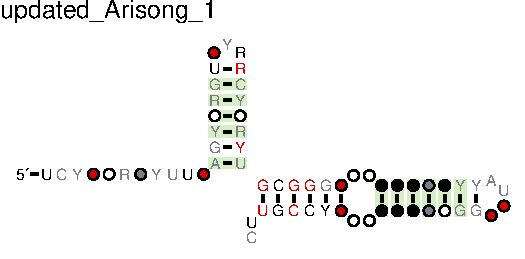
\includegraphics[scale=1.5]{Arisong_R2R.pdf} 
 \caption{\small\textbf{\emprog{tutorial/updated\_Arisong\_1.R2R.sto.\{pdf,svg\}}:
     annotated consensus secondary structure.} Base pairs with
   covariation scores equal or below the target E-value (0.05 as
   default) are depicted in green. By default only positions in the
   alignment with more than 50\% occupancy are depicted (unless they form
   a base pair). Option \prog{--r2rall} forces the depiction of all
   positions in the alignment.  }
 \label{fig:r2r}
 \end{figure}

 \begin{figure}
   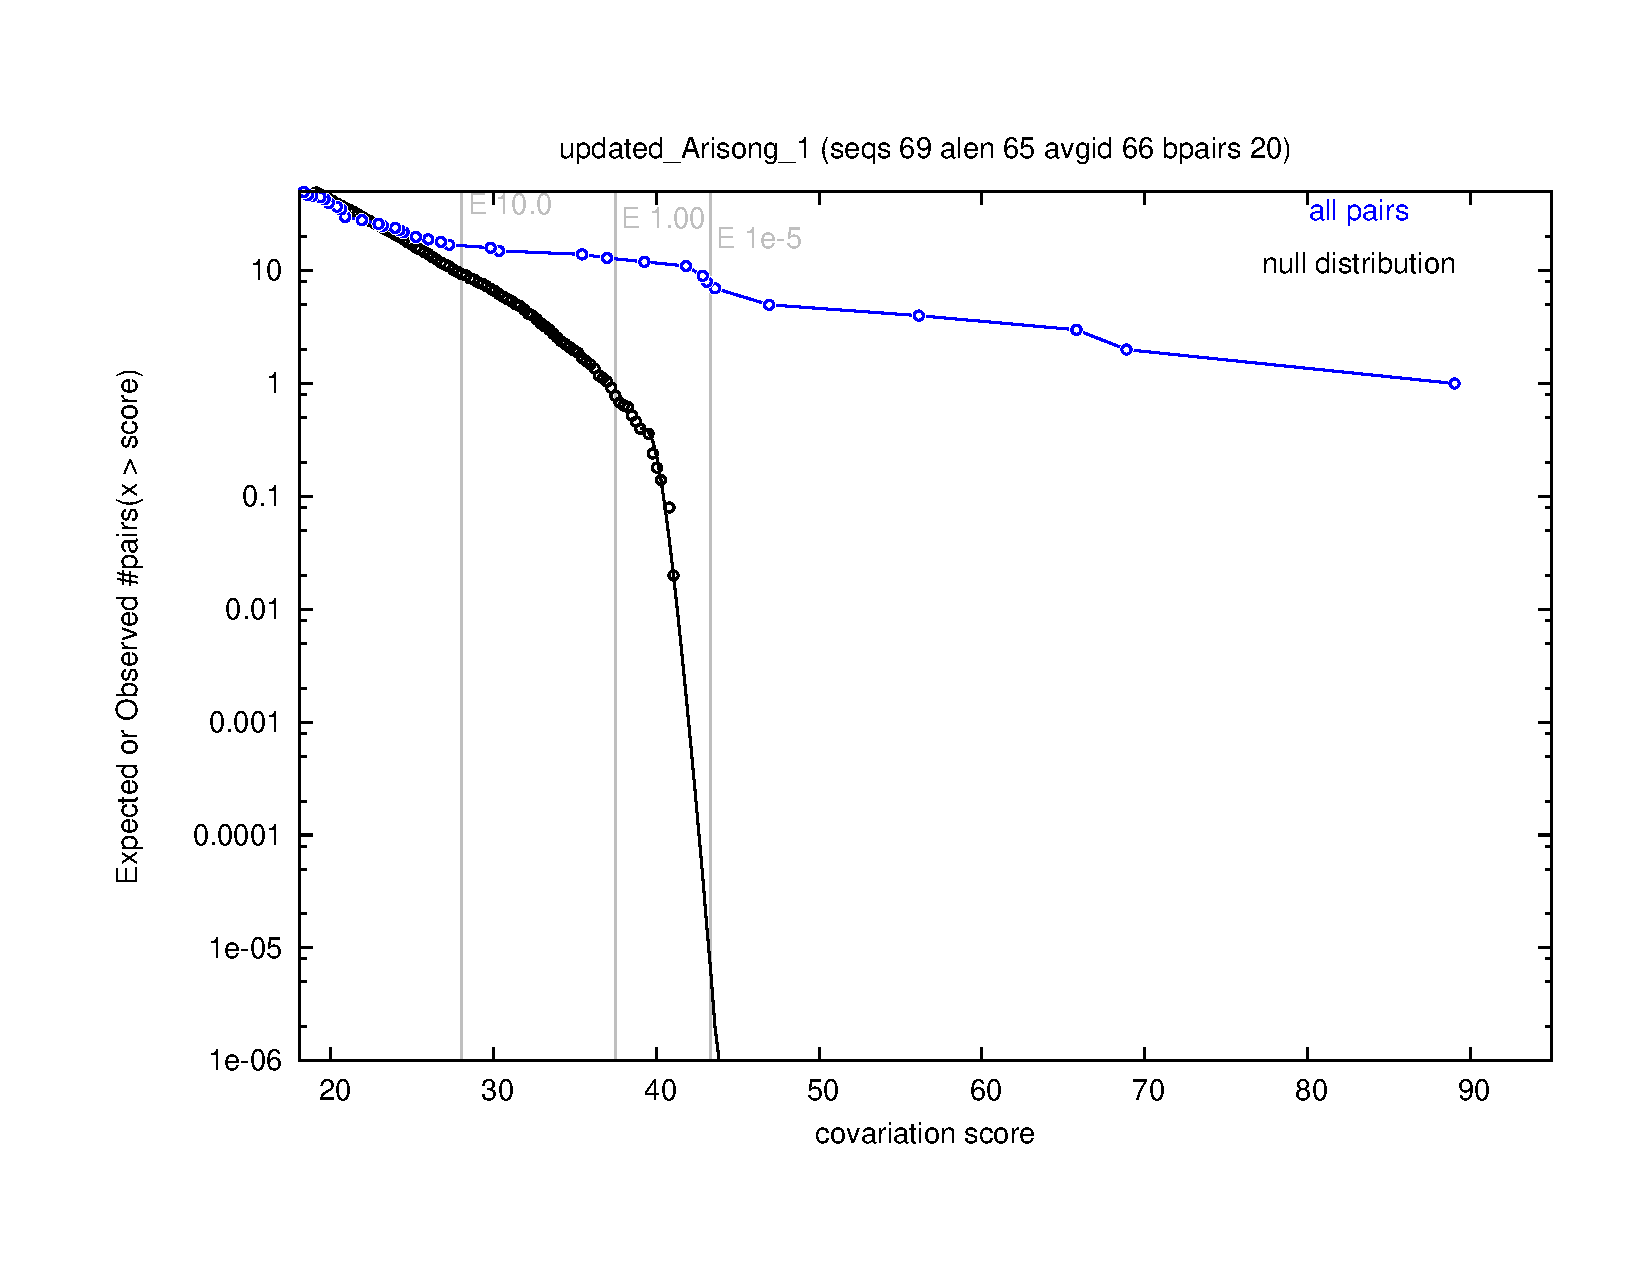
\includegraphics[scale=0.50]{Arisong_his.pdf} 
 \caption{\small\textbf{\emprog{tutorial/updated\_Arisong\_1.his.\{ps,svg\}}:
     covariation scores histogram.}  The histogram of scores for all
   pairs in the given alignment is depicted in blue. The histogram for
   the null alignments is depicted in black. A black line indicates to
   fit to a truncated Gamma distribution of the tail of the null
   distribution. In red, we plot the histogram of scores for the pairs
   in the given alignment excluding those proposed as base pairs.}
 \label{fig:histogram}
 \end{figure}


 \begin{figure}
   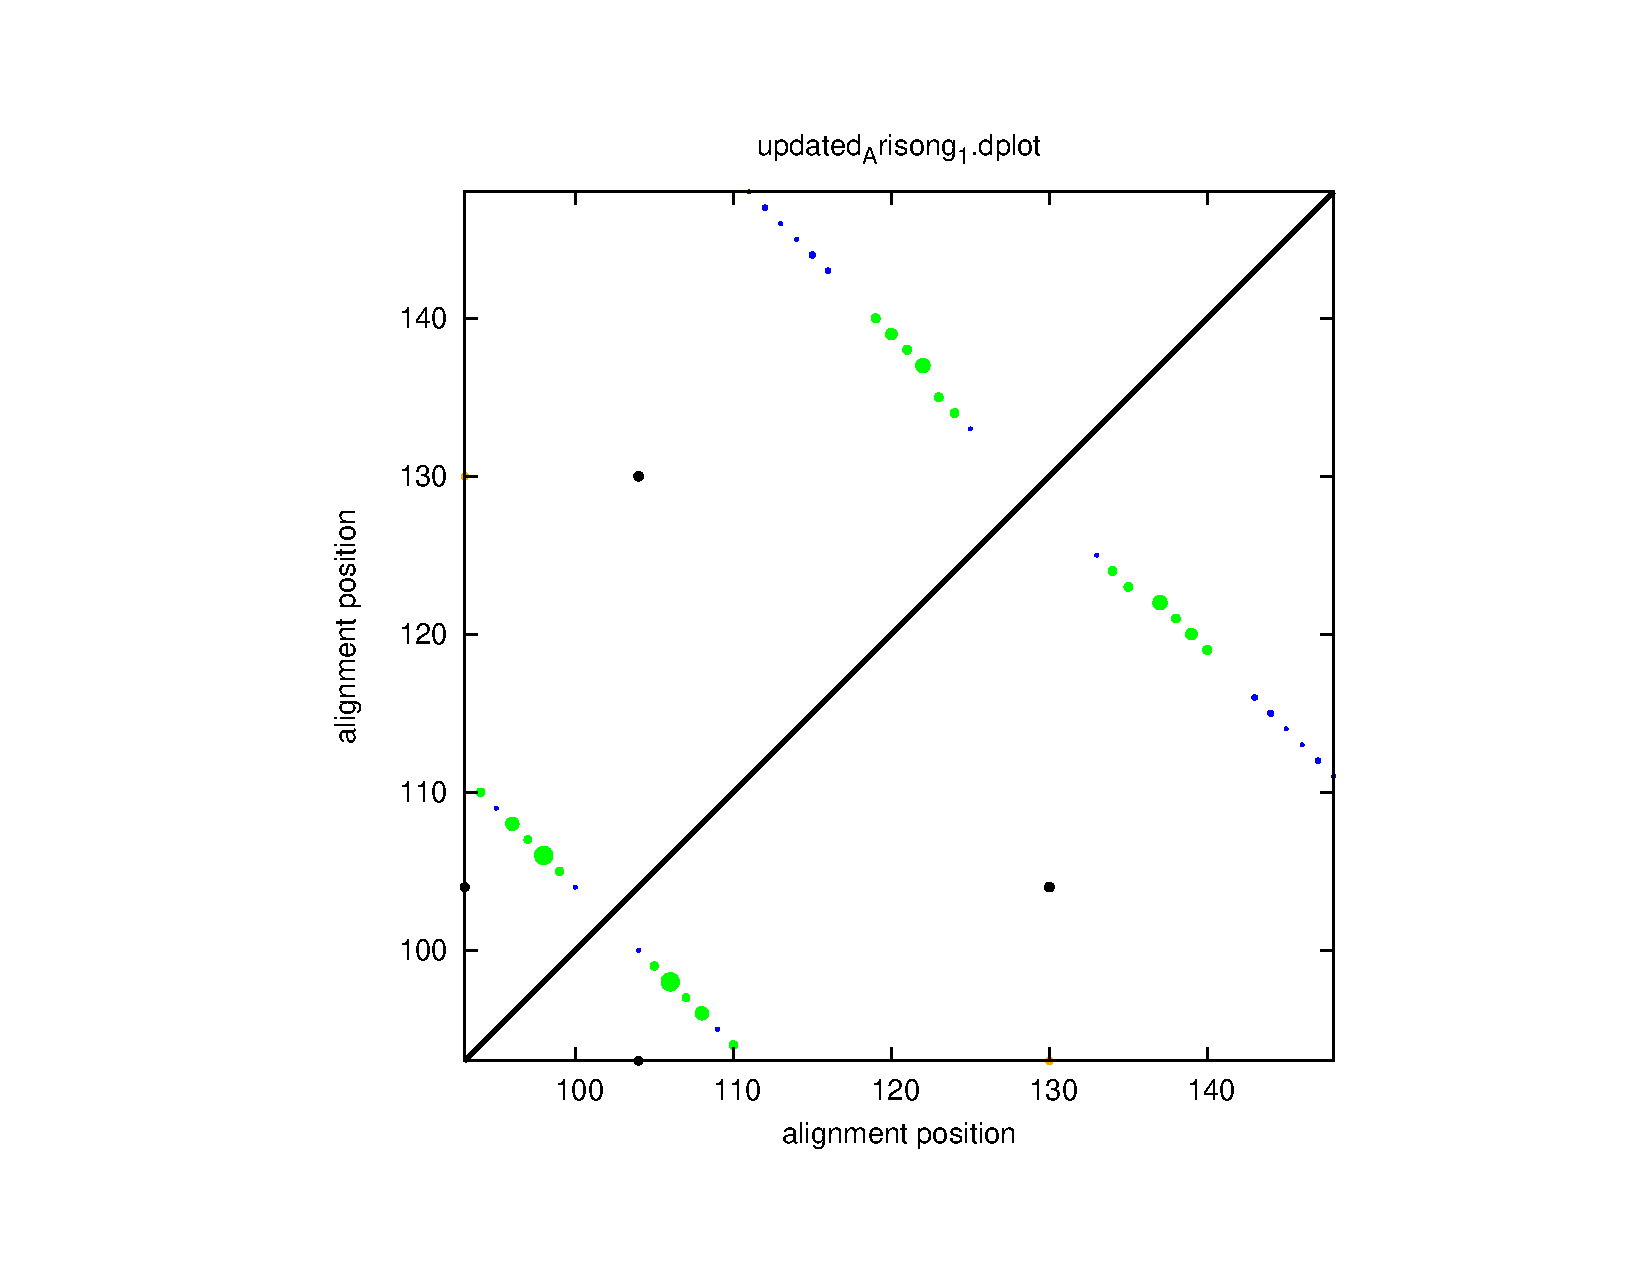
\includegraphics[scale=0.60]{Arisong_dplot.pdf}
 \caption{\small\textbf{\emprog{tutorial/updated\_Arisong\_1.dplot.\{ps,svg\}}:
     dotplot.}  Dot size is proportional to the covariation score. In
   blue we depict the consensus base pairs; in green, the consensus
   base pairs that show significant covariation; in orange (none shown
   in this plot), we depict other pairs that have significant
   covariation, are not part of the consensus secondary structure but
   are compatible with it; in black we depict other significant pairs.
   Position are relative to the input alignment}
 \label{fig:dplot}
 \end{figure}



 \clearpage
 \subsection{Other tabular outputs}

 \rscape\ produces two more tabular outputs per input file that are
 more relevant for benchmarking purposes, those are:\\

 File \emprog{tutorial/updated\_Arisong.sum} looks lie:

 \begin{sreoutput}
 more tutorial/updated_Arisong.sum 
 #target_E-val   MSA                     nseq    alen    avgid    method  TP      True    Found   SEN     PPV
 0.050000        updated_Arisong_1       69      65      65.16    GTp     9       20      20      45.00   45.00 
 \end{sreoutput}
 This file produces a one line output per alignment in the file.
 \begin{sreitems}{\prog{Second column}}
 \item[\prog{Column 1}] Target E-value.
 \item[\prog{Column 2}] Alignment name.
 \item[\prog{Column 3}] Number of sequence in the analyzed alignment.
 \item[\prog{Column 4}] Number of columns analyzed.
 \item[\prog{Column 5}] Average percentage identity in the analyzed alignment.
 \item[\prog{Column 6}] Covariation statistic.
 \item[\prog{Column 7}] Number of significant base pairs (tf).
 \item[\prog{Column 8}] Number of base pairs (true).
 \item[\prog{Column 9}] Number of significant pairs (found).
 \item[\prog{Column 10}] Sensitivity = tf/true.
 \item[\prog{Column 11}] Positive predictive value = tf/found.

 \end{sreitems}

 File \emprog{tutorial/updated\_Arisong.roc} looks like:
 \begin{sreoutput}
 more tutorial/updated_Arisong.roc
# MSA nseq 69 alen 65 avgid 65.163163 nbpairs 20 (20)
# Method: GTp
#cov_score  FP  TP  Found  True  Negatives   Sen   PPV     F       E-value
89.04630    0   1       1    20       2060   5.00  100.00  9.52    0
88.79103    0   1       1    20       2060   5.00  100.00  9.52    0
88.53575    0   1       1    20       2060   5.00  100.00  9.52    0
...
\end{sreoutput}

This file produces a tabular output for each alignment and for as a
function of the covariation score. The values in the file are
described by the commented line.
